% Generated by scripts/make_measurement_tables.py; do not edit.
\begin{table}[htbp]
\centering\small
\begin{tabular}{@{}rrrrrr@{}}
\toprule
$t$ & Dense variables & Kernel variables & Kernel (ms) & Dense (ms) & Paired ratio \\
\midrule
4 & 17 & 6 & 0.338 & 1.430 & 4.24 \\
8 & 33 & 6 & 0.580 & 6.569 & 11.05 \\
16 & 65 & 6 & 1.567 & 36.457 & 23.55 \\
32 & 129 & 6 & 1.864 & 104.015 & 58.70 \\
64 & 257 & 6 & 3.859 & 400.672 & 108.13 \\
128 & 513 & 6 & 7.391 & 1,850.127 & 251.63 \\
\bottomrule
\end{tabular}
\caption{The identical fixed-sector Q-ray task on boundary-cap triangulations.
Every case has $k=d=1$. Times are medians of ten measured calls per method;
the last column is the median of ten within-round dense/kernel ratios.
The comparator is the independent dense Python reference.}
\label{tab:sparsebench}
\end{table}

\begin{table}[htbp]
\centering\small
\begin{tabular}{@{}rrrrr@{}}
\toprule
$t=k$ & Maximum coordinate bits & Certificate bytes & Median (s) & Measured calls \\
\midrule
4 & 3 & 4,747 & 0.006032 & 10 \\
8 & 6 & 10,700 & 0.010546 & 10 \\
16 & 11 & 32,752 & 0.042811 & 10 \\
32 & 22 & 117,706 & 0.226509 & 10 \\
64 & 44 & 455,055 & 1.542706 & 10 \\
128 & 89 & 1,792,597 & 11.075735 & 6 \\
\bottomrule
\end{tabular}
\caption{Complete certified discovery on supplied dense Fibonacci sectors.
All have $d=1$ and return one verified essential meridian.
The clock includes native independent disc replay and JSON serialization.
These are timings of the new method, without a cross-algorithm ratio.}
\label{tab:fibbench}
\end{table}

\begin{figure}[htbp]
\centering
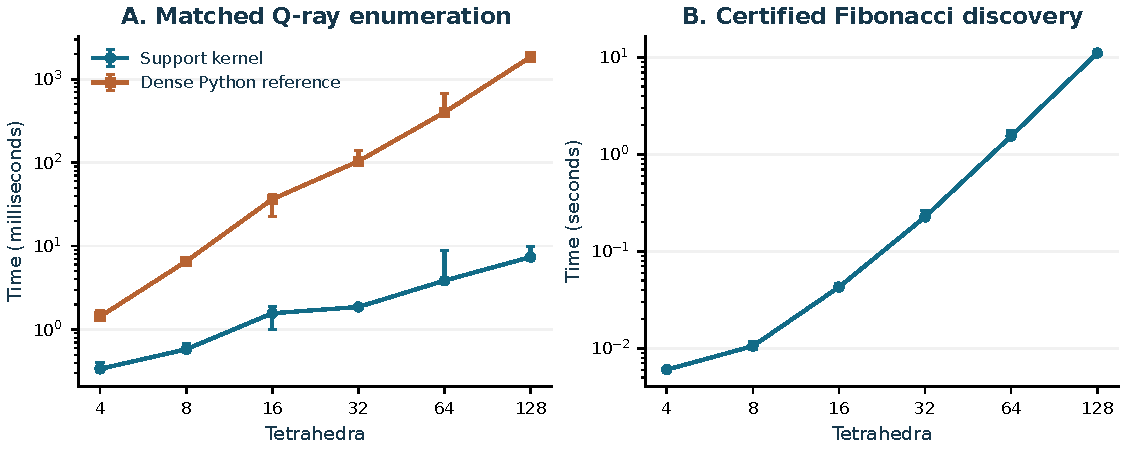
\includegraphics[width=\textwidth]{benchmark_scaling.pdf}
\caption{Measured scaling for two different supplied-sector workloads.
Points are medians; bars span the observed minimum and maximum.
Both axes are logarithmic. The bars describe repeat variability,
not confidence intervals or a distribution over inputs.}
\label{fig:bench}
\end{figure}

The main run completed 176 measured calls and
36 retained warm-up calls on Python 3.12.14.
The frozen runtime and benchmark source hashes were unchanged from the
beginning to the end of that run. A first exploratory timing run is also
retained separately; the tables use only the second, controlled run.
No other agent computation was scheduled concurrently with this main run.
